\documentclass{article}
\usepackage[utf8]{inputenc}

%---------------------------------------------------
%
%---------------------------------------------------

\usepackage{amsmath}
\usepackage{amssymb}
\usepackage{blindtext}
\usepackage{bm}
\usepackage{float}
\usepackage[margin=.75in]{geometry}
\usepackage{graphicx}
\usepackage{mathrsfs}
\usepackage{multicol}

\def\changemargin#1#2{\list{}{\rightmargin#2\leftmargin#1}\item[]}
\let\endchangemargin=\endlist

\renewenvironment{abstract}
{
\begin{changemargin}{0.5in}{0.5in}
}
{
\end{changemargin}
}

\newcounter{theorems}
\newenvironment{theorem}
{
\stepcounter{theorems}
\begin{changemargin}{0.25in}{0.25in}
\noindent
\textbf{Theorem \arabic{theorems}:}
\begin{em}
}
{
\end{em}
\end{changemargin}
}


\newenvironment{proof}
{
\begin{changemargin}{0.25in}{0.25in}
\noindent
\textbf{Proof: }
}
{
\begin{flushright}
$\blacksquare$
\end{flushright}
\end{changemargin}
}

%---------------------------------------------------
%
%---------------------------------------------------

\title{Run AwAI: StarCraftII Adversary Avoidance Using Neural Networks and
  Genetic Algorithms}

\author{Kyle R. Chickering \\ krchicke@ucdavis.edu
  \and Alex R. Mirov \\ armirov@ucdavis.edu
  \and Simon H. Wu \\ simwu@ucdavis.edu
  \and Xin Jin \\ jin@ucdavis.edu}

\date{June 8, 2018}

%% TODO: Why our approach vs other approaches
%% TODO: Random action is a fairly robust approach to the problem space
%% TODO: Include convergence Graphs in the results section
%% TODO: Talk about the mutation rates in the genetic algorithm
%% TODO: Reference the fact that neuro evolution is good in high dimensional
%%    and continuous state spaces (ref neat paper)

\begin{document}

\maketitle
\hline
\\~\\

\begin{abstract}
  \textbf{Abstract}: \blindtext
  \\~\\
  \textbf{Keywords}: Machine Learning, Genetic Algorithms, Neural Networks,
  StarCraftII
\end{abstract}
\\~\\
\hline
\\~\\

\begin{multicols}{2}
\section{Introduction}
Since AlphaGo's defeat of the Go champion Ke Jie, the artificial intelligence
community has
been looking for the next problem domain to apply learning techniques to. A
potentially surprising candidate for artificial intelligence testing has
emerged in the form of real time strategy games. Real time strategy games work
by having a player make critical decisions in real time against an enemy
player. The game StarCraftII, released by Blizzard entertainment in 2010, is a
real time strategy
game that has captured the interest of the artificial intelligence community.
The game presents several challenges for artificial intelligence, the biggest of
which is the magnitude of possible game states.

We present a method of teaching an agent to avoid enemy players for as long as
possible by using genetic algorithms to evolve neural networks. We interface
our neural network agents using the PySC2 library  and evolve an agent that
shows a measurable increase in its ability to run away.

\section{Background}
This project combines two proven artificial intelligence paradigms: neural
networks and genetic algorithms. These methods are traditionally orthogonal,
but there has been a growing body of work in recent years with regards to
evolving neural networks using genetic algorithms. Most notably \cite{NEAT} and
[ref].

\subsection{Neural Networks}
Neural networks are a method of computing any computable function by using a
network of nodes called \textbf{neurons} connected by a series of edges. This
representation is inspired by the human brain, and has been proven over and over
as a heavy hitter in the world of machine learning. These networks are typically
differentiable, and by calculating error, they can be trained using a method
called backpropogation that changes the strength of the connections between
neurons.

There are two main ways to represent neural networks in software, implicitly and
explicitly. Implicit neural networks use linear algebra and a consistent layered
structure to propagate inputs forward (called feeding forward). With numerical
linear algebra libraries available for almost every major programming language,
this method of representing neural networks allows for incredibly fast
processing
of neural networks. However, this representation's greatest strength, its speed,
is the source of its greatest weakness. Implicitly defined neural networks
suffer
from the inflexibility of their layered structure. In the human brain, neurons
are not limited to any specific structure, and are free to make connections
that could not be possible in a layered model.

This leads us to explicitly defined neural networks. These networks allow the
specification of new nodes that are disconnected from the traditional layered
model. While this can be advantageous, it can also present problems for the
implementer. Because these models are represented by graphs, we can no longer
use linear algebra libraries to feed forward through the network. This causes
an increase (often significant) in running time. For small networks this is
not an issue, but for larger network this becomes (sometimes prohibitively)
problematic.

\subsection{Genetic Algorithms}
In a similar line of though that led researchers to build neural networks by
looking to nature for inspiration, genetic algorithms exploit natural selection
to create optimal solutions to problems. Research into genetic algorithms
started when researchers realized that there is nothing inherent in evolution
that limits the process to nature . In fact, by thinking of evolution as
an algorithm in and of itself, we can extend the principle of evolution to
digital systems. This is commonly done by defining what an "individual" and
"fitness function" mean in the digital evolution landscape. The algorithm
proceeds as evolution does in nature by picking the most well adapted
individuals to "breed", and evaluating their "offspring" on the same problem.
This technique has yielded several fascinating results, and often the
algorithm generates novel solutions to difficult problems.

\section{Methodology}
Our approach involved combining genetic algorithms and neural networks to
create an agent that learns through evolution how to evade antagonistic
agents. We chose this method as the problem space closely resembles nature's
predator/prey motif. By modeling our agent as an evolving neural network we can
get results that mimic generational evolution in nature. While evasion,
especially in the StarCraftII space, is a fairly simple behavior, we chose this
method as it is easily extendable to larger problem spaces by extending the
input and output dimensions.

There are many techniques to accomplish running away from enemies in
StarCraftII, for example, a simple expert system would be quite good at enemy
avoidance, however we were concerned with the scalability of our approach. We
chose the neural network and genetic algorithm approach because for dealing
with more complex tasks, our approach is more robust than a simple expert
system. Additionally, we could train various neural networks on different
tasks (avoidance, attacking, resource mining, etc.) and splice the neural
networks together to build an AI capable of multitasking during the game.

By introducing scalability, we could use our existing framework to train neural
networks in more and more difficult simulated environments, eventually leading
to an AI that could play the entire game outside of sandbox mode. Neural
networks generalize very well to a wide array of situations that are similar or
close to the situations they were trained on, and they are a perfect tool for
attacking a game that requires real time decision making and reasoning over a
complex set of inputs.

\subsection{Simulations}
To compute the fitness for each neural network in the population, we run the
network through a simulation. The simulation is run in StarCraftII, and our
simulation controller is built on top of the PySCII interface, and simulates
a ``game'' with our agent and a group of adversaries, which are controlled by
the in game AI that come with the game.

Each simulation is called an episode, and we ran the networks through 5-10
episodes each so that we could get a representative sample of the amount of time
that each neural network was able to survive.

We let the neural network choose the next action from our action space, which
consists of a series of movement directions (eight cardinals and a stay
command).

\begin{figure}[H]
\centering
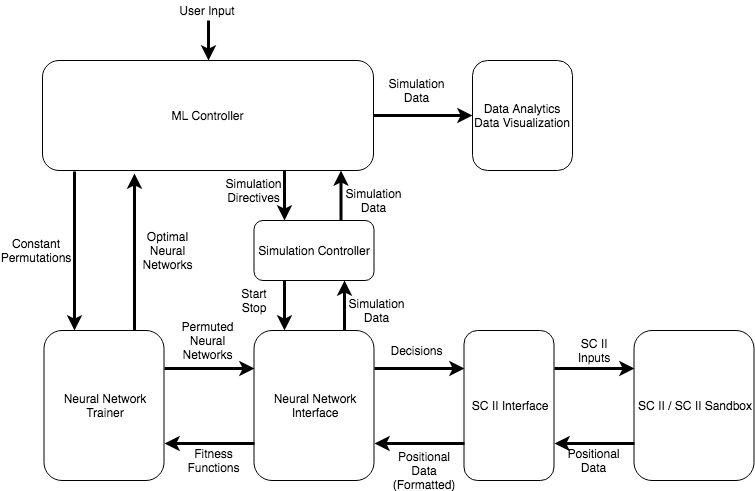
\includegraphics[width=0.45\textwidth]{chart}
\begin{changemargin}{0.15in}{0.15in}
  \caption{Control and data flow through the Run AwAI controller.}
\end{changemargin}
\end{figure}

Talk about the mathematical model we are using to run the simulations

\subsection{Neural Network}
We started by using an explicit neural network implementation, which we chose
because we were curious if the flexible topologies would lead to a more
efficient neural network. We were inspired by the NEAT algorithm \cite{NEAT}, which has
shown promise in other video game domains. However we choose a simpler
topologically explicit implementation to simplify the development of our
algorithm. We ultimately settled on an acyclic graph representation, which
allowed us the freedom to add nodes and allowed simple manipulation of
connection weights.

We chose to use our neural network to represent a function taking an input
vector consisting of relative agent position and adversary's relative position
and return an output vector of directions.
\begin{align}
  \bm{V} = \mathcal{N}(\bm{I})
\end{align}
Where $\mathcal{N}$ is the function computed by our neural network. We choose
the next action according to the equation:
\begin{align}
  a_n = \max_{v \in \bm{V}} \: v
\end{align}
This input vector is flexible, and allows us to tweak the information that we
feed to the neural network. Additionally, while the output space we used
contains only movement in the cardinal directions, we could easily add other
supported actions like attacking and mining resources.

Our network uses the standard sigmoid function $\varsigma$ as its activation
function:
\begin{align*}
  \varsigma(x) = \frac{1}{1 + e^{-x}}
\end{align*}
We chose this function for a number of reasons, the least of which is its
popularity as an activation function in neural networks. Because of the shape
of the sigmoid function, inputs to subsequent neurons stay in the nice range of
$[-1, 1]$, which has the effect of normalizing the network. Since we are not
using backpropogation, the nice properties of the sigmoid function were
unimportant to us. However, if we were to do live backpropogation during
simulations, the sigmoid function would be a useful activation function.

When we initialize the network, we populate all of the connection weights from
a random Gaussian distribution with $\sigma = 1$ and $\mu = 0$. This serves to
make our input data ``nice'' for the sigmoid function, which ends up returning
either $1$ or $-1$ when the input data is amplified by non-gaussian data. This
also ensures that most connections are ``off'' or close to off at the start,
which allows the network to learn without any random pre-bias. Our first
generation will have very weak suggestions on the effectiveness of the next
move. This may seem bad, but it allows us to do much slower mutation changes to
the connection weights, which in turn increases the explorative power of our
algorithm. If the weights are too heavy in the beginning, the agent will favor
a local maximum almost immediately, but with a Gaussian distribution, the
algorithm explores more options before settling on a specific maximum.

\subsection{Genetic Algorithm}
For our implementation, we used a tournament style selection process to choose
our most fit individuals. We use tournament selection over other selection
methods (like probabilistic selection), to improve convergence speeds.
Tournament selection is an exploitive selection method, and we choose exploitive
behavior over exploratory behavior because our simulation was a substantial
bottleneck in our iterative process. Because we choose an exploitive method, we
limit the chances of finding a global maximum, but increase the chances of
finding some local maximum, and finding it relatively quickly. This gave us a
chance to better observe the convergence of our algorithm, and allowed us to
demonstrate clear forward progress.

To get convergence, we spent a lot of time looking at fitness functions. We
considered many different
possibilities, but finally settled on a measure of the number of steps that our
agent took during the simulation. We figured that this would be a good measure
of our agent's ability to stay alive, and we thought that time alive was a good
indicator of the agent's ability to accomplish the goal of running away. We
computed the fitness $F$ using the following formula:
% \begin{align}
%   F(\bm{i}) = \mu - \eta\sqrt{\frac{1}{|\bm{\mathcal{E}}|}
%   \sum_{e \in \bm{\mathcal{E}}}\left(\mathcal{S}(e) - \mu\right)^2} 
% \end{align}
% where
% \begin{align}
%   \mu = \frac{1}{|\bm{\mathcal{E}}|} \sum_{e \in \bm{\mathcal{E}}} \mathcal{S}(e)
    %   \end{align}
\begin{align}\label{eq:fitness}
  F(\bm{i}) = \frac{1}{|\bm{\mathcal{E}}|} \sum_{e \in \bm{\mathcal{E}}} \mathcal{S}(e) - \eta\sqrt{\frac{1}{|\bm{\mathcal{E}}|}
   \sum_{e \in \bm{\mathcal{E}}}\left(\mathcal{S}(e) - \frac{1}{|\bm{\mathcal{E}}|} \sum_{e \in \bm{\mathcal{E}}} \mathcal{S}(e)\right)^2} 
\end{align}
and $\bm{\mathcal{E}}$ is the set of all episodes run by the PySCII simulation,
$\mathcal{S}(e)$ is the number of steps taken by the agent in the episode, and
$\bm{i}$ is a an individual of the population. $\eta$ is a hyper-parameter we
use
to fine tune the convergence of our network. We are effectively calculating the
average number of steps and penalizing the individuals based on the standard
deviation from the mean of the episodes. This serves to mitigate the effects
presented by individuals that get ``lucky'' and have a good trial runs that
offsets their average.

We seed the evolutionary controller using $n$ random individuals, and in each
evolutionary iteration, we breed $n\text{C}2$ individuals to compose the
subsequent generation. After breeding, we randomly mutate some of the children,
and then calculate the fitness for each individual in the population. To get
the next generation, we choose the most fit $n$ individuals from the population
to breed, and repeat the cycle. In addition, we found that the algorithm
converged more rapidly if we let the most fit individuals survive to the next
generation, and after making this change we noticed a jump in convergence
speeds.

The genetic algorithm relies on several hyper-parameters. The most obvious is
the
population size. We find, unsurprisingly, that larger population sizes are more
robust and generate faster convergence, this makes sense because with larger
population sizes there is an increased chance of mutation, and mutations are
largely responsible for exploratory behavior in learning algorithms. We have
three mutation parameters, which are the rate at which nodes are added to the
network, the rate at which new connections are added to the network, and the
rate at which connection weights are changed.

We mutate connection rates based on a Gaussian distribution, which, combined
with our Gaussian weight initialization, ensures that weights never change
dramatically. We adjust weights according to the formula:
\begin{align}
  w_i \leftarrow w_i + \bm{\sigma}
\end{align}
where $\bm{\sigma}$ is a random variable from a Gaussian distribution.

\subsection{Controller}

\subsection{PySC2 Interface}
Our simulation learning environment was based on an existing environment
included in the PySC2 library\cite{pysc2}. We use the ``Defeat Roaches'' mini
game as the baseline for our learning. Once we had the map, we used the
StarCraftII map editor to tweak the mini game to better suit our needs. We
created three maps that were used in testing. The defualt map is a simple square
map which spawns a group of adversarialy ``roaches'', and a group of ``marines'',
who are controlled by our agent. The marines and roaches are spawned in the
same place every time, which gives us a consistent platform to test our agent.

The second variation is similar to the first, except that there is only one
``roach'' and one ``marine''. This map type highlights the capabilities of our
agent in a more intimate setting. The group of marines has the advantage of
being able to get ``lucky'' and have some members survive, but the 1v1
variation forces the neural network to work well from the beginning.

All maps were edited in the SCII map editor. 

\subsubsection{Learning Environment}
The final map chosen for our simulations was the default DefeatRoaches mini game. The mini game provides a simple map that is 64x64 without any obstacles that spawns a group of marines and roaches at two spawn points within the map. 

\subsubsection{Map Variations}
DefeatRoaches 1v1 - 
Similar to the default DefeatRoaches map except for the number of marines and 
roaches in the map at spawn time. This custom map only has 1 marine and 1 roach at the designated spawn points. 

The decision to make this custom map was made early on to make the learning environment as simple as possible for training purposes.

DefeatRoaches96 - 
This variation, DefeatRoaches96, is a 96x96 map that is bigger than the original. This allows the agent to have a larger input space to choose from which could potentially improve rate of convergence to an optimal solution. 

\section{Results}
We ran several simulations with various choices of hyperparameters, and our
results are promising. We saw measurable improvement in preformence after just
a few iterations of the algorithm, which gave us a steep initial learning curve
before the improvements started to taper off.

\begin{figure}[H]\label{fig:fitness graph}
\centering
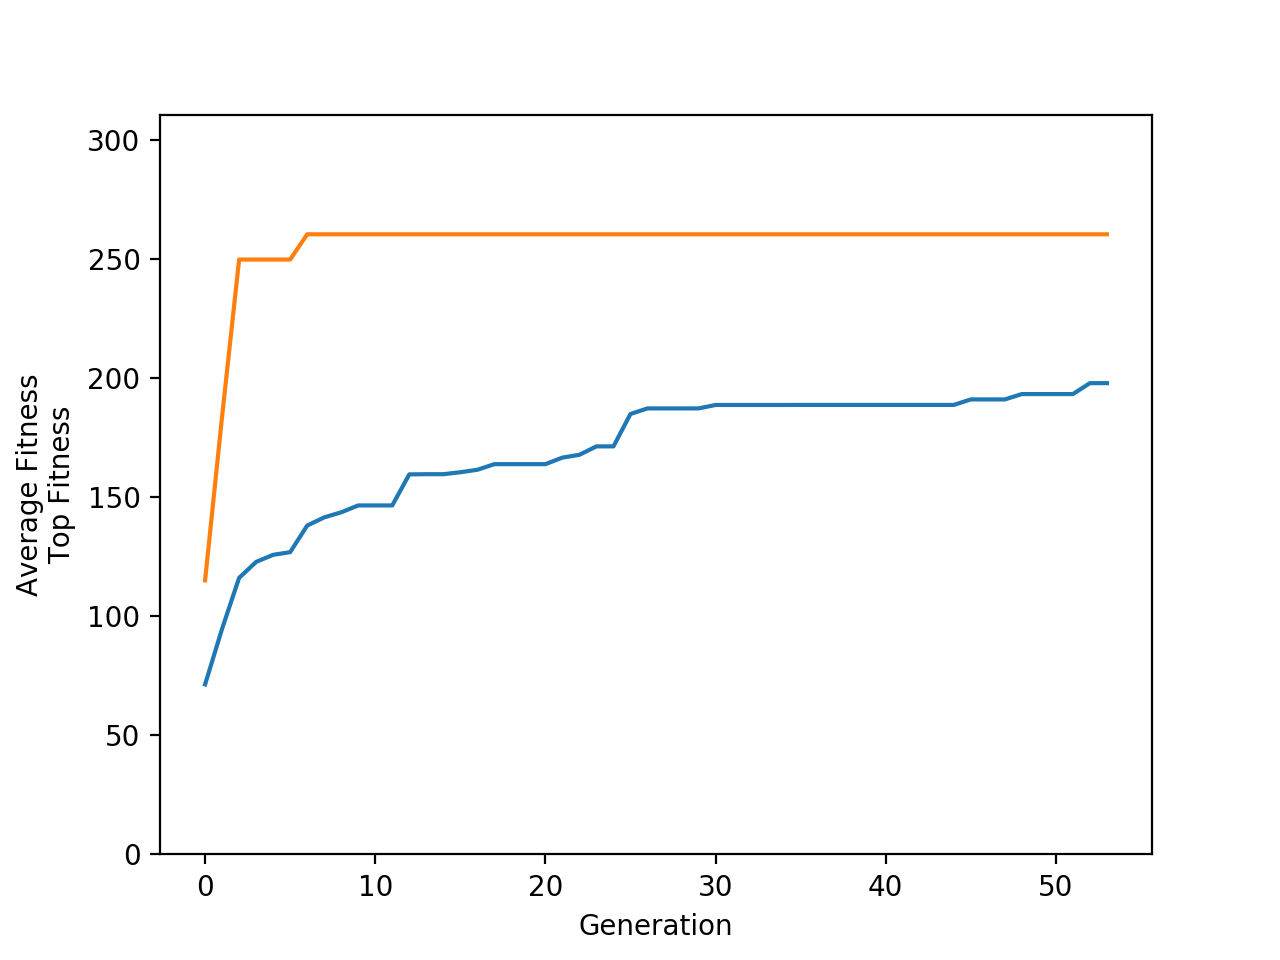
\includegraphics[width=0.45\textwidth]{fig_1}
\begin{changemargin}{0.15in}{0.15in}
  \caption{Graph of average fitness (blue) and top fitness (orange) for each
    generation in Trial 1. Top fitness is the fitness of the most fit individual
    at the end of each generation's simulations. Average fitness is calculated
    by averaging \eqref{eq:fitness} over all individuals $\bm{i}$ in the
    population. The breeding constant is set to 15, node generation rate is set
    to 0.3, new connections at 0.2 and non structural mutations at a rate of
    0.4}
\end{changemargin}
\end{figure}

We see in Figure \ref{fig:fitness graph} an artifact from our choice of genetic
algorithm. Because we keep the top individual from each generation in the gene
pool, we see that the top individual has palteaued early, and no new individual
is achieving a higer fitness. We see that the average is countinually decreasing
though, which will increase the chances that an individual will be bred that has
a higher fitness than the individual that is dominating the maximum fitness.

We can also see that the average sometimes plateaus as well. This is due to a
homonginization of the gene pool, where the children individuals are very
similar to their parents. This is a case of finding a local maximum. Since we
favored an exploitive algorithm, this is to be expected, however we see that the
population can still achieve higher fitness meausures which means that the
algorithm still retains some amount of exploratory behavior.

\begin{figure}[H]\label{fig:fitness graph}
\centering
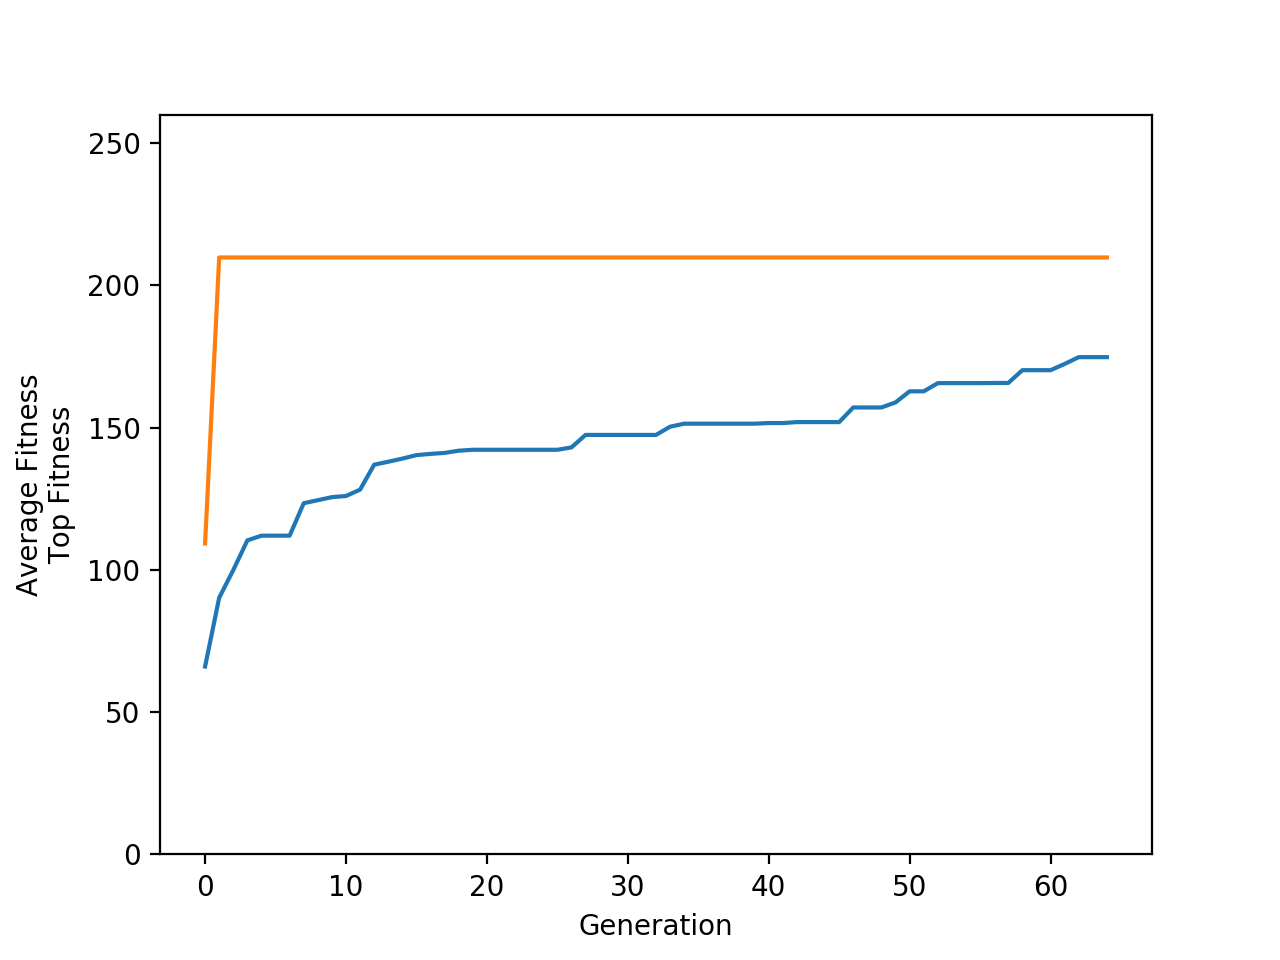
\includegraphics[width=0.45\textwidth]{fig_2}
\begin{changemargin}{0.15in}{0.15in}
  \caption{Graph of average fitness (blue) and top fitness (orange) for each
    generation in Trial 1. Top fitness is the fitness of the most fit individual
    at the end of each generation's simulations. Average fitness is calculated
    by averaging \eqref{eq:fitness} over all individuals $\bm{i}$ in the
    population. The breeding constant is set to 15, node generation rate is set
    to 0.5, new connections at 0.5 and non structural mutations at a rate of
    0.75}
\end{changemargin}
\end{figure}

In our second trial, we see that the average fitness increases much more
regularly. However, despite having more generations, trial two did not reach the
same average fitness as trial one did. One possible reason for this is since our
mutation rates are higher, our algorithm favored a more exploratory approach,
which lead to a more consistant incresase in fitness, but did not reach as high
of an average fitness.

%% TODO: Talk about choice of hyper paramters, population size, episode count
%% mutation constants, eta in fitness function

\section{Conclusion}
Different selection types?
\blindtext

\subsection{Improvements}
\blindtext
\blindtext

\subsection{Future Work}
This project can certainly be extended in many ways, for example, we could
extend the output vectors to include offinsive manuvering by our agent, and
train the agent to be agressive by considering the number of adversaries killed
by our agent during the simulation.

Another possibility that we did not explore, was the effect of removing neurons
from the network. Neural networks can often be plauged by overfitting input
data, and by removing neurons we hypothesize that any overfitting we encounter
could be mitigated. We would remove these neurons in the same way that we add
neurons, that is, non-deterministically as a possible mutation. In the study of
biological creatures, we often see either total dropping of traits from the
population genome or the transition to vestigial genetic structure
\cite{lehman}. In keeping with this, instead of outright removing the neuron, we
could significantly decrease the strength of the connections to it, essentially
removing it from the network. If the neuron in question was indeed problematic,
we would see it countinue to evolve very low weights, essentially pruning the
neuron and rendering it vestigial.

We could also track the lifespan of certain individuals and kill them off after
a certain number of generations. We found that the algorithm would sometimes
plateau with a very fit individual for a period of time, and it would be
interesting to see what effects a notion of ``lifetime'' would have on the
algorithm as a whole.

\end{multicols}

\\~\\
\hline
\\~\\

\begin{thebibliography}{9}
\bibitem{NEAT} 
  Kenneth O. Stanley, Risto Miikkulainen.
  \textit{Evolving Neural Networks through Augmenting Topologies}. 
  The MIT Press Journals.

\bibitem{dejong}
  Kenneth A. De Jong. \textit{Evolutionary Computation: A Unified Approach}.
  MIT Press, Feb 3, 2006.

\bibitem{russell}
  Stuart Russell, Peter Norvig.
  \textit{Artificial Intelligence: A Modern Approach}.
  Upper Saddle River (New Jersey, 1995).

\bibitem{lehman}
  Joel Lehman et al.
  \textit{The Surprising Creativity of Digital Evolution: A Collection of
    Anecdotes from the Evolutionary Computation and Artificial Life Research
    Communities}.
  \textbf{https://arxiv.org/pdf/1803.03453.pdf}.

\bibitem{pysc2}
  Google DeepMind pysc2.
  \textbf{https://github.com/deepmind/pysc2}.

\end{thebibliography}

\end{document}